\chapter{Programming - Automatic Cutting Sequence}
\section{Best Practices}\paragraph*{Block cut programming}can be a lengthy process, with frequent interruptions at times. Using the \textbf{CHECK PROGRAM} screens (Chapter 9, Check Program Screens) to verify where you left off is an easy way to continue programming from the correct spot. If you combine this with stroking out, or otherwise indicating completion point on your Operation Sheets, is a good double check practice to use. When starting a new program for cutting blocks with the saw, it is always a good idea to follow these few steps at first ...
\begin{list}{$\diamond$}{}
	\item \textbf{Reset Automatic Sequence}
	\item \textbf{Clear Block Program}
	\item \textbf{Home Saw}
\end{list}
This will ensure the system is ready to start "fresh" with a new program to execute (once the Operator enters it). 
\section{Saw Program Details}\paragraph*{Programming the Saw} is done by the Operator through entering relevant data via the combination of screens provided. (Refer to chapters 7-9 for details on how to). The block data entered by the Operator is the cut program for the saw. The automatic execution of the block cutting program is done by the saw, according to a sequence that combines the Block and Slab information as entered by the Operator, and executes the command sequence as described below. A repeating cycle of ...
\begin{list}{$\diamond$}{}
	\item \textbf{Move (Long Travel) to cut location, whether \textit{First Cut} or not}
	\item \textbf{Saw through block at this location using a repeating forward and backward motion of the Cross Travel while lowering vertical by the drop amount after each pass. Also maintaining at or below the current setting of the saw motor as set by the Operator}
	\item \textbf{Raise Vertical to Home}
	\item \textbf{Index Long to next cut position} (if there are more blocks, if not cycle is complete and the \textit{Automatic Sequence} is stopped (\textit{Cycle Stop}) and the \textit{Block Program} data is cleared)
	\item \textbf{Repeat sawing operation}
\end{list}
The saw can be programmed to cut from one to two hundred blocks with zero to five hundred slabs total. While this is beyond the physical limits of the working envelope of the saw, it does afford flexibility to the Operator when programming. A block can have zero slabs, which is a block to be cut in two. A block can have up to five different sized slabs each with their own respective quantities, if it is large enough. 
\paragraph{\textbf{\LARGE \textcolor{blue}{i}}}It's also good practice to take the time during any settings changes, either program type, or operation type, to allow for the communication process between the PLC and HMI to complete. In the case of most settings there is a standard request for change then change complete response which takes place. This causes observable delays from the Operators point of view. Although this time is merely seconds at worst, when in the "heat" of work, and pressed for time, it may seem to drag on. Upon \textit{Automatic Program} cycle completion, the \textit{Block Program} data is cleared by having 0 written to every memory location where \textit{Block and Slab Program} data is stored in the controller.
\paragraph*{Programming the Saw - Vertical Travel Details}Figure 10.1 is a simplistic diagram to show the relative dimensions that comprise the vertical axis travel limits. The Vertical Axis, Long Axis, and Cross Travel Axis, limits are combined to derive the working envelope of the saw. In Figure 10.1, the vertical travel is shown as the dimension \textit{b}. While dimension \textit{a} is the maximum forward limit as set by the \textit{Forward Limit Proximity Sensor}. Currently the home position of the Vertical Axis is hard set at 38.25 inches from the ground. The forward limit can change in order to accommodate variations in the wooden cribbing that supports the stone blocks being cut. As mentioned this change is accomplished by adjusting the \textit{Forward Limit Proximity Sensor} to suit. The immediate thing of note, would be the actual block height that can be accommodated by this saw (dimension \textit{b}) which would be 38.25"- \textit{dim a} - \textit{safety gap(if desired)}. In the notes above about the sequence of operation during automatic cycle, it is worth noting the first cut, from the Vertical Axis POV. When the Long Travel has completed moving to the position commanded, whether first or later cuts on the same block, the vertical will be commanded to move to the \textit{Block Height}, then to the \textit{current height} - \textit{Cut Depth} as programmed by the operator. The second motion command is actually the beginning (in the Automatic Program) of the sawing motion loop. This will usually result in a noticeable pause when starting each new sawing motion. Subsequent Vertical Axis motion until the current cut location is completed, is determined by simply \textit{Position} = \textit{current height} - \textit{Cut Depth}. At the end of each cut, when the final pass completes, the \textit{Vertical Axis} is returned to it Home position, fully raised. This position, fully raised, is the only position of the vertical axis that the program will allow the Long travel to move.
\paragraph{\textbf{\LARGE \textcolor{blue}{i}}}Each cut is a series of passes of the \textit{Cross Travel Axis} \textbf{after} the \textit{Vertical Axis} has lowered by the \textit{Cut Depth} setting amount. when doing a first pass of the cutting motion at a new \textit{Cut Location}, there are two \textit{Vertical Axis} moves commanded ...
\begin{list}{$\diamond$}{}
	\item \textbf{move to \textit{Block Height}} then ...
	\item \textbf{move to (\textit{Current Height} - \textit{Cut Depth})}
\end{list}
When programming \textit{Block Height}, it is strongly recommended to pick the highest point of the block. It is worth noting that \textit{Block Height} is the dimension from the floor (not the top of the cribbing) to the top of the block.
\begin{figure}
	\centering
	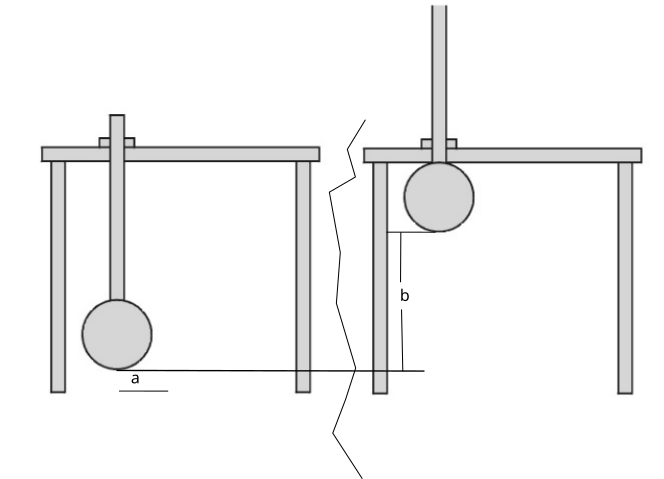
\includegraphics[width=0.5\linewidth]{screen-captures/program/kodiak-saw-vert-travel}
	\caption{Programming - Vertical Travel}
	\label{fig:prg-vert-travel}
\end{figure}
\newpage
\paragraph*{Programming the Saw - Cross Travel Details}Figure 10.2 is a simplistic diagram to show the dimensions that comprise the cross travel axis travel limits. The  \textit{Cross Travel Axis}, during Automatic sequence, will travel to \textit{Forward Position} then back to \textit{Home} while the sawing action is being performed on the stone block. The \textit{Forward Position} is the position where the saw blade will clear the stone block. The Maximum Speed of the \textit{Cross Travel Axis} is determined by the \textit{Cut Depth} the Operator has programmed and a formula based upon how much material the saw blade and segments can remove at nominal motor RPM. The speed through the stone, and the load on the saw blade, is further affected by adjusting the \textit{Motor Current Setting}, which is directly tied to the PID process variable. This allows the Operator to make adjustments for stone hardness for example. There is also a programmable speed override which can be enabled which is intended to be used by the Operator when new segments have been installed and the blade needs to be run in at a low speed. This setting is password protected with a time limit on entry. When in automatic and running a program, the \textit{Cross Travel Axis} will try to travel at the programmed speed as determined by the calculation that uses the \textit{Cut Depth Setting}, also while trying to maintain the \textit{Motor Current Setting}, and the \textit{Speed Override} as the limit set by the Operator, will take precedence over all speed control while it is enabled.
\paragraph{\textbf{\LARGE \textcolor{blue}{i}}}If the Operator finds the saw to be working too much while in the stone, lowering the \textit{Motor Current Setting} may help. If the saw is moving through the stone without reaching the current setting, then increasing the \textit{Cut Depth} may be required. It is important for longevity of the segments to make sure and disable the speed override once the segments have opened up after run in of new ones.
\begin{figure}
	\centering
	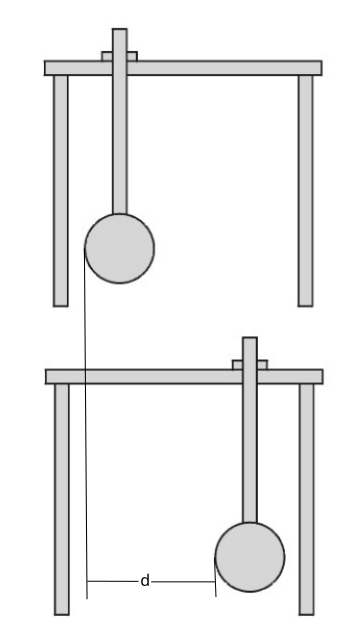
\includegraphics[width=0.3
	\linewidth]{screen-captures/program/kodiak-saw-crosst-travel}
	\caption{Programming - Cross Travel}
	\label{fig:prg-cross-travel}
\end{figure}
\newpage
\paragraph*{Programming the Saw - Long Travel Details}Figure 10.3 is a simplistic diagram to show the relative dimensions that comprise the long travel axis travel limits. The left hand side is representing the Home position of the Long Travel Axis, and the right hand shows the saw with it's Long Travel Axis in the forward limit position. The Long Travel Axis moves from the Home Position to towards the Forward Position during automatic block cutting in order to eliminate any potential backlash in the rack and pinion drive of the axis, which could introduce inaccuracies in position and or it's repeatable capabilities. The dimension \textit{e} is the maximum forward travel in inches, for the Long Travel Axis. The Long Travel Axis, is commanded to move to the \textit{First Cut} location of each block that is programmed by the Operator. The \textit{Automatic Program} begins by loading the \textit{First Cut} location for the (current) block, and instructing the Long Travel Axis to move to that location (which may be 0 for the first block). Once the first cut is completed, the \textit{Automatic Program} will check to see if there are any slabs to cut for the currently loaded block. If there is one or more slabs (size) of one or more quantity, then the Automatic Program will add the \textit{Slab Size} (Chapter 8, Block Program) plus the \textit{Blade Kerf} (Chapter 7, Saw Parameters) to the \textit{current Long Travel} position, and load the new position into the \textit{Long Travel Axis} index command position and trigger the index move. If there are more than one of this size of slab, the quantity counter is reduced by one at this time. If there is no other slab quantity of this slab, then once the cut has completed the Automatic Program checks for more slabs for this block, finding none will result in this block being \textit{marked complete} in the program temporary memory. The \textit{Automatic Program} will load the next \textit{Slab Data} until there are no more slabs for this block. At that moment, at cut complete for the final slab of the current block, the \textit{Automatic Program} will check for any more block data to load. If there are more blocks, the cycle returns to loading the next block data, then moving to \textit{First Cut} of the (now current) block. If, however there are no more blocks to cut, the program is marked complete in internal memory storage once the \textit{Vertical Axis} returns to it's home position.
\paragraph{\textbf{\LARGE \textcolor{blue}{i}}}The \textit{Long Travel Axis} is the axis that is most important to dimensional accuracy of the end product. It is therefore important to maintain the travel rails for this axis clean and debris free to ensure unimpeded movement. When programming positions into the \textit{Block Program} it is very important to always start from the \textit{Home} position moving towards the \textit{Forward Limit} to ensure the rack and pinion drives backlash does not affect the position being set/recorded. Tape measures are great verification tools.
\begin{figure}
	\centering
	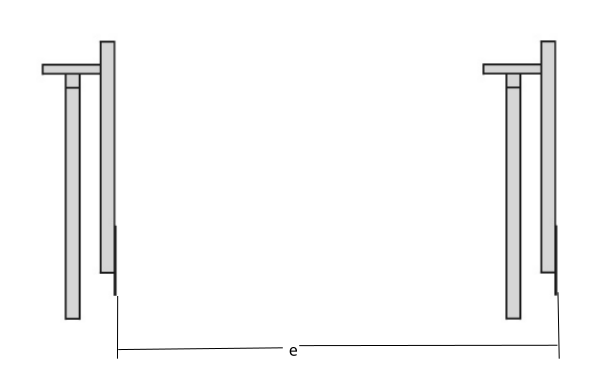
\includegraphics[width=0.5\linewidth]{screen-captures/program/kodiak-saw-long-travel}
	\caption{Programming - Long Travel}
	\label{fig:prg-long-travel}
\end{figure}